
\subsection{Procedure}
There are a few constraints and conditions that must be followed in order for the analytical 
function to work with SWIRL, 

\begin{itemize}
    \item The mean flow and speed of sound must be real and positive. This will 
        occur is a speed of sound is chosen such that the tangential mach number
        is imaginary
    \item The derivative of the speed of sound must be positive
    \item Any bounding constants used with the mean flow should not allow the 
        total Mach number to exceed one.
    \item the speed of sound should be one at the outer radius of the cylinder
\end{itemize}

Given these constraints, $tanh(r)$ is chosen as a function since it can be
modified to meet the conditions above. Literature (The tanh method: A tool for 
solving certain classes of nonlinear evolution and wave equations) 
is a paper than demonstrates the strength of using tanh functions.
One additonal benefit of tanh(r) is that it is bounded between one and negative one, i.e.

\begin{itemize}
    \item As r $\rightarrow$ $\infty$ tanh(r) $\rightarrow$ 1
    \item As -r $\rightarrow$ $-\infty$ tanh(r) $\rightarrow$ -1
\end{itemize}

To test the numerical integration method,  $M_{\theta}$ is defined as a result 
of differentiating the speed of sound, $A$. This is done opposed to integrating
$M_{\theta}$ analytically. However, an analytical function can be defined for
$M_{\theta}$, which can then be integrated to find what $\widetilde{A}$ should be. 
Instead, the procedure of choice is to back calculate what the appropriate 
$M_{\theta}$ is for a given expression for $\widetilde{A}$.  Since it is easier 
to take derivatives , we will solve for $M_{\theta}$ using Equation \ref{eq:Mthetabackcalculated} ,

\subsection{Tanh Summaion Formulation}
Knupp's Code Verification by the Method of Manufactured Solution (MMS) provides 
``guidelines'' for creating a manufactured solution (MS) such that the observed
order of accuracy will approach a theoretical order of accuracy as the number
of grid points are reduced from one iteration to the next. While these guidelines
offer a road map, there are choices that are left to the investigator that would
benefit from additional examples. The first guideline gives the user a free
choice of the MS as long as it s smooth. The benefit of the tanh summation method 
(TSM) reduces the difficuly in defining a sufficient MS by providing 
a general summation formulation that allows the user to Vary the number of 
terms in the MS, and the MS behavior without manually changing terms in the MS
symbolic expression. 

The general form of the MS will be a summation of $tanh$ bounded between zero
and one. A MS created with the TSM can provide a significant result for
a numerical differencing/integration technique by having inflection points of each
$tanh$ at various locations along the domain, giving a stair like slope.
While the TSM can add a layer of complexity to the MS that may not be needed, 
writing the formulation in a summation lends itself to iterative loops that can 
be coded, thus reducing the need for manual adjust of the MS, 
which can be an initial hurdle when performing MMS.


\section{General form of a Hyperbolic Tangent}

\begin{equation}
    R = A tanh(B(x-C)) 
    \label{eqn:1}
\end{equation}

\begin{equation}
    L = A tanh(B(C-E)) 
    \label{eqn:2}
\end{equation}
\begin{equation}
    y = R + L + D
    \label{eqn:3}
\end{equation}
where 
\begin{itemize}
    \item $R \equiv$ The value of the hyperbolic tangent. The variable $R$ represnts
        a ``right'' facing hyperbolic tangent kink.
    \item $A \equiv$ magnitude factor that increases or decreases the asymptotic
        limits $\lim_{x \to -\infty} = -1$ $\lim_{x \to \infty} = 1$
    \item $B \equiv$ ``steepness'' of the hyperbolic tangent
    \item $C \equiv$ The shift in inflection point of the hyperbolic tangent along the $
        x$ axis 
    \item $D \equiv$ The shift in inflection point of the hyperbolic tangent along the $
        y$ axis 
    \item $E \equiv$  $x_{i=i_{max}}$
    \item $x$ The domain. $x_i$ is used to indicate grid point indicies.
\end{itemize}
The idea is to sum up an arbitrary amount of tangents that will be bounded by zero
and one. 

\begin{figure}
    \centering
    \resizebox{\columnwidth}{!}{
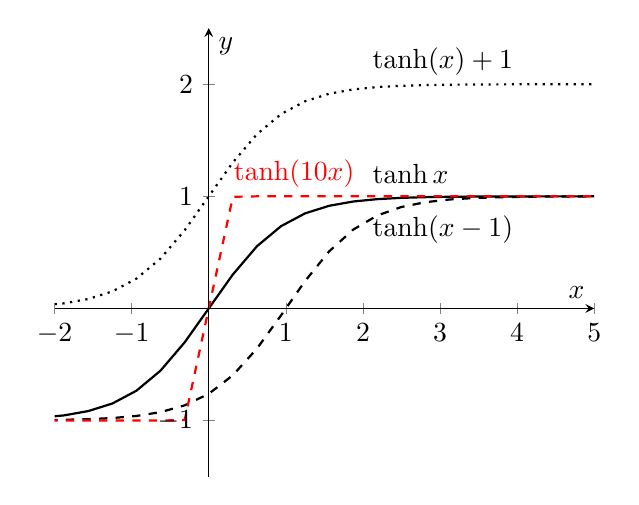
\begin{tikzpicture}
    \begin{axis}[
        xmin=-2, xmax=5,
        ymin=-1.5, ymax=2.5,
        axis lines=center,
        axis on top=true,
        domain=-2.5:5,
        ylabel=$y$,
        xlabel=$x$,
        ]

        \addplot [mark=none,draw= black, thick] {tanh(\x)};
        \node [right, black ] at (axis cs: 2,1.2) {$ \tanh x$};


        \addplot [mark=none,draw=black, dashed, thick] {tanh(\x - 1)};
        \node [right, black] at (axis cs: 2,0.7) {$ \tanh (x - 1)$};



        \addplot [mark=none,draw=red, dashed, thick] {tanh(10*\x)};
        \node [right, red] at (axis cs: 0.2,1.2) {$ \tanh (10x )$};



        \addplot [mark=none,draw=black, dotted, thick] {tanh(\x) + 1};
        \node [right, black] at (axis cs: 2,2.2) {$ \tanh (x) + 1$};

    \end{axis}
\end{tikzpicture}}
\end{figure}


Now the goal is to generalize this formulation such that we can add up terms.
$A$ is determined by setting a maximum amplitude for each $tanh$ function by
$A = A_{max}/n$. Note that amplitude can be different for each term but is chosen
to be the same. A parameter $\hat{x} = (x - x_{min})/ (x_{max} - x_{min}$ scales the domain to be between the  
minimum and maximum bounds.


\begin{equation}
    R_{ij} = A tanh(B(x_i-C_j)) 
    \label{eqn:1}
\end{equation}

\begin{equation}
    L_{j} = A tanh(B(C_j-E)) 
    \label{eqn:2}
\end{equation}
\begin{equation}
    y = \sum_{j = 1}^{n}  R_{ij} + \sum_{j = 1}^{n}L + D
    \label{eqn:3}
\end{equation}
The function \verb|TanhMethod| does this procedure. 

Setting $A = 1/16$ and $C_1  = 0$ , $C_2 = 0.75$ , $C_3 = 1$ , $D = 1$, $E = 1$  and 
$B = 10$


\begin{equation}
    \sum_{j = 1}^{3} R_{ij} = 1/16 tanh(10(\hat{x}_i))  + 1/16 tanh(10(\hat{x}_i-0.75)) + 1/16 tanh(10(\hat{x}_i-1))
    \label{eqn:1}
\end{equation}

\begin{equation}
    \sum_{j = 1}^{3} L_{j} = 1/16 tanh(10(-1))  + 1/16 tanh(10(0.75 - 1)) + 1/16 tanh(10(1-1))
    \label{eqn:1}
\end{equation}

The simplified expression becomes,
\begin{equation}
    y = \frac{1}{16}\tanh\left(\frac{100}{9}r - \frac{100}{9}\right) + \frac{1}{16}\tanh\left(\frac{100}{9}r -\frac{55}{9}\right) + \frac{1}{16}\tanh\left(\frac{100}{9}r -\frac{10}{9} \right) + \frac{7}{8}
\end{equation}


%\begin{figure}
%    \centering
%    \resizebox{\columnwidth}{!}{
%% This file was created with tikzplotlib v0.10.1.
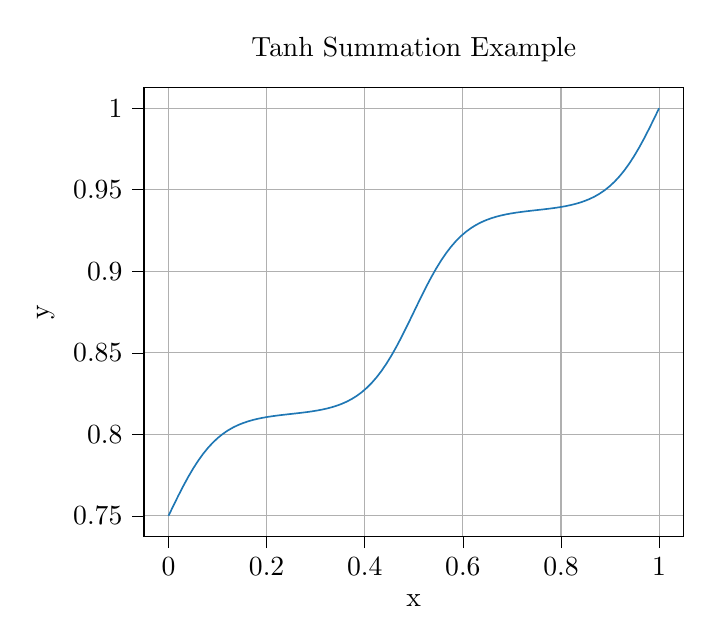
\begin{tikzpicture}

\definecolor{darkgray176}{RGB}{176,176,176}
\definecolor{steelblue31119180}{RGB}{31,119,180}

\begin{axis}[
tick align=outside,
tick pos=left,
title={Tanh Summation Example},
x grid style={darkgray176},
xlabel={x},
xmajorgrids,
xmin=-0.05, xmax=1.05,
xtick style={color=black},
y grid style={darkgray176},
ylabel={y},
ymajorgrids,
ymin=0.737511917481587, ymax=1.01249943250088,
ytick style={color=black}
]
\addplot [semithick, steelblue31119180]
table {%
0 0.750011349982464
0.0101010101010101 0.756304367923548
0.0202020202020202 0.762471427961815
0.0303030303030303 0.768396284241735
0.0404040404040404 0.773980954849054
0.0505050505050505 0.779151246168556
0.0606060606060606 0.78385900159005
0.0707070707070707 0.788081304133098
0.0808080808080808 0.791817372304981
0.0909090909090909 0.795084105493723
0.101010101010101 0.797911187966577
0.111111111111111 0.80033644822293
0.121212121212121 0.802401902498815
0.131313131313131 0.804150668035091
0.141414141414141 0.805624753143957
0.151515151515152 0.806863623924088
0.161616161616162 0.807903399550648
0.171717171717172 0.808776520778204
0.181818181818182 0.809511752175423
0.191919191919192 0.810134404577104
0.202020202020202 0.810666691986701
0.212121212121212 0.811128162249061
0.222222222222222 0.811536161419119
0.232323232323232 0.81190630759737
0.242424242424242 0.812252961565677
0.252525252525253 0.812589689584715
0.262626262626263 0.812929718947268
0.272727272727273 0.813286389915873
0.282828282828283 0.813673608902656
0.292929292929293 0.814106307344292
0.303030303030303 0.814600908628971
0.313131313131313 0.815175801361504
0.323232323232323 0.815851810708233
0.333333333333333 0.816652649865894
0.343434343434343 0.817605320080265
0.353535353535354 0.81874040944222
0.363636363636364 0.820092217733837
0.373737373737374 0.82169860781786
0.383838383838384 0.82360045643945
0.393939393939394 0.825840555061835
0.404040404040404 0.828461805118854
0.414141414141414 0.831504577298413
0.424242424242424 0.835003179865009
0.434343434343434 0.838981523240156
0.444444444444444 0.84344828154901
0.454545454545455 0.848392114910775
0.464646464646465 0.853777768834061
0.474747474747475 0.859544011154561
0.484848484848485 0.865604291561671
0.494949494949495 0.871850642171087
0.505050505050505 0.878160707811378
0.515151515151515 0.884407058420794
0.525252525252525 0.890467338827903
0.535353535353535 0.896233581148403
0.545454545454546 0.901619235071689
0.555555555555556 0.906563068433454
0.565656565656566 0.911029826742308
0.575757575757576 0.915008170117455
0.585858585858586 0.918506772684051
0.595959595959596 0.92154954486361
0.606060606060606 0.924170794920629
0.616161616161616 0.926410893543014
0.626262626262626 0.928312742164604
0.636363636363636 0.929919132248627
0.646464646464647 0.931270940540244
0.656565656565657 0.9324060299022
0.666666666666667 0.93335870011657
0.676767676767677 0.934159539274231
0.686868686868687 0.93483554862096
0.696969696969697 0.935410441353493
0.707070707070707 0.935905042638172
0.717171717171717 0.936337741079808
0.727272727272727 0.936724960066591
0.737373737373737 0.937081631035197
0.747474747474748 0.937421660397749
0.757575757575758 0.937758388416787
0.767676767676768 0.938105042385094
0.777777777777778 0.938475188563345
0.787878787878788 0.938883187733403
0.797979797979798 0.939344657995763
0.808080808080808 0.939876945405361
0.818181818181818 0.940499597807041
0.828282828282828 0.94123482920426
0.838383838383838 0.942107950431816
0.848484848484849 0.943147726058376
0.858585858585859 0.944386596838507
0.868686868686869 0.945860681947373
0.878787878787879 0.947609447483649
0.888888888888889 0.949674901759534
0.898989898989899 0.952100162015887
0.909090909090909 0.954927244488741
0.919191919191919 0.958193977677483
0.929292929292929 0.961930045849366
0.939393939393939 0.966152348392414
0.94949494949495 0.970860103813909
0.95959595959596 0.97603039513341
0.96969696969697 0.981615065740729
0.97979797979798 0.98753992202065
0.98989898989899 0.993706982058916
1 1
};
\end{axis}

\end{tikzpicture}

%}
%\end{figure}
%The goal is generate an MS with a number of ``stairs'' that is bounded between
%zero and one. Here's what my focus group ideas are,
%
%\begin{align*}
%    1 = R + L 
%\end{align*}
%where, 1 is a constraint, and R and L are the two waves when summed need to cancel 
%if it were the exact same amplitude \& opposite sign 
%
%so ,
%
%\begin{align*}
%    R + L = \tanh(x) + -\tanh(x) = 0
%\end{align*}
%or in our case,
%
%\begin{align*}
%    R + L = \tanh(x) + -\tanh(x) = 1
%\end{align*}
%
%We can tweak this by adding knobs by adding ``knobs'' A and B. If we dont want 
%the total to not exceed one then, $A_j + A_{j+1} \cdots A_{last} = 1$. $B_1$ changes
%the steepnes of the kink that we want. In order to generalize this,
%
%
%\begin{align*}
%    \bar{A} = \sum_{j=1}^n R_{ij} + \sum_{j=1}^n L_{ij} 
%\end{align*}
%where,
%\begin{align*}
%    R_{ij} = A_j \tanh(B_j (x_i - x_j)) \\ 
%    L_{ij} = A_j \tanh(B_j (x_j - x_n))  
%\end{align*}
%
%Letting $n = 3 \ldots$
%
%\begin{align*}
%    \bar{A} &= S_{vert} + \sum_{j=1}^3 R_{ij} + \sum_{j=1}^3 L_{ij} \\
%    \bar{A} &=
%    A_1 \tanh(B_1 (x_i - x_1))  + 
%    A_{2} \tanh(B_{2} (x_i - x_{2}))  + 
%    A_{3} \tanh(B_{3} (x_i - x_3)) +  \\
%    A_1 \tanh(B_1 (x_1 - x_n)) &+ 
%    A_{2} \tanh(B_{2} (x_2 - x_{n}))  +
%    A_{3} \tanh(B_{3} (x_3 - x_n))  
%\end{align*}
%and,
%\begin{align*}
%    A_1 = A_2 = A_3 = k_1 \\ 
%    B_1 = B_2 = B_3 = k_2  
%\end{align*}
%
A tanh summation method was constructed to make a manufactured solution with 
strong changes in slope. This ensures that the numerical approximation will not 
give trivial answers. 
then for some functions we need to impose boundary conditions. We will demonstrate
how the careless implementation of a boundary condition can lead to close approximations
on the interior.  The speed of sound is defined with the subscript $analytic$ to indicate that this is the analytical function of choice and has no physical relevance 
to the actual problem.

\begin{align*}
\widetilde{A}_{analytic} = \Lambda + k_1 \tanh \left( k_2 \left( \widetilde{r} - \widetilde{r}_{max} \right) \right),
\end{align*}

where, 

\begin{align*}
    \Lambda = 1 - k_1 \tanh(k_2 (1 - \widetilde{r}_{max})),
\end{align*}

When, $\widetilde{r}=\widetilde{r}_{max}$ , $\widetilde{A}_{analytic} = 1$.  
Taking the derivative with respect to $\widetilde{r}$,

\begin{align*}
    \frac{\partial \widetilde{A}_{analytic} }{\partial \widetilde{r}} &=
    \left(1 - \tanh^{2}{\left(\left(r - r_{max}\right) {k}_{2} \right)}\right) {k}_{1} {k}_{2}, \\ 
    &= \frac{ k_{1} k_{2}}{\cosh^{2}{\left(\left(r - r_{max}\right) {k}_{2} \right)}}.
\end{align*}

Substitute this into the expression for $M_{\theta}$ in Equation 
\ref{eq:Mthetabackcalculated},

\begin{align*}
    M_{\theta} = \sqrt{2}
    \sqrt{\frac{r {k}_{1} {k}_{2}}{\left(\kappa - 1\right) \left(\tanh{\left(\left(r - r_{max}\right) {k}_{2} \right)} {k}_{1} + \tanh{\left(\left(r_{max} - 1\right) {k}_{2} \right)} {k}_{1} + 1\right) \cosh^{2}{\left(\left(r - r_{max}\right) {k}_{2} \right)}}}
\end{align*} 

Now that the mean flow is defined, the integration method used to obtain the 
speed of sound

% What happens when $r = r_{max}$?

Initially the source terms were defined without mention of the indices of the 
matrices they make up. In other words, there was no fore sight on the fact that
these source terms are sums of the elements within A,B, and X. To investigate 
the source terms in greater detail, the FORTRAN code that calls the source 
terms will output the terms within the source term and then sum them, instead 


of just their sum.
i
$ [A]{x} = \lambda [B] {x} $

which can be rearranged as,

$ [A]{x} - \lambda [B] {x} = 0$

Here, $x$ is an eigenvector composed of the perturbation variables, $v_r,v_{\theta},v_x,p$ and $\lambda$ is the associated eigenvalue, (Note: $\lambda = -i \bar{\gamma}$)

Writing this out we obtain $\cdots$.

Linear System of Equations:
\begin{equation}
    -
    i \left(
        \frac{k}{A} - \frac{m}{r} M_{\theta}
    \right)
    v_r 
    -
    \frac{2}{r} M_{\theta} v_{\theta} 
    +
    \frac{dp}{dr} 
    +
    \frac{(\kappa - 1)}{r} M_{\theta}^2 p
    -
    \lambda M_x v_r =S_1
\end{equation}

Using matrix notation,

\begin{equation}
    A_{11}
    x_1 
    -
    A_{12} x_2 
    +
    A_{14} x_4
    -
    \lambda B_{11} x_1 = S_1
\end{equation}


But $A_{14}$ and $A_{41}$ in Kousen's paper only has the derivative operator.
Since I am currntly writing the matrix out term by term and not doing the matrix 
math to obtain the symbolic expressions, I will define $A_{14}$ with $dp/dr$ 
and $A_{41}$ with $dv_r/dr$
Similarly,
\begin{align}
    A_{21} x_1 &-
    A_{22} x_2 +
    A_{24} x_4 &-
    \lambda B_{22} x_2 &= S_2 \\
    A_{31} x_1 &-
    A_{33} x_3 &-
    \lambda (B_{33} x_3 + B_{34} x_4) &= S_3\\
    A_{41} x_1 &+
    A_{42} x_2 +
    A_{44} x_4 &- 
    \lambda (B_{33} x_3 + B_{44} x_4) &= S_4
\end{align}
Now we can begin looking at the source terms, term by term. They each should also
converge at a known rate





